\chapter{Experiment Design, Theory, and Results}

Verifying millimeter-wavelength absorption spectrum of SO$_2$ is important for the study of the atmosphere of Venus. Making measurements under simulated Venus conditions assures the accuracy of any model derived from such measurements.
 Described below is the theory, laboratory equipment, measurement procedure and derived uncertainties in the measurements of the millimeter-wavelength absorptivity of gaseous sulfur dioxide under simulated Venus conditions.

\section{Measurement Theory}

In this experimental program, quality factor (Q) of a resonant mode of a resonator is used to measure the absorption of a gas or gas mixture \cite{high-sensitivity}. The quality factor of a resonance is given by \cite{matching}

\begin{equation} \label{eq:qlong}
Q = \frac{2\pi f_0 \textnormal{ x Energy Stored}}{\textnormal{Average Power Loss}}
\end{equation}

\noindent where $f_0$ is the resonant frequency. The Q of a resonance can be measured directly from $f_0$ by dividing it by its half-power bandwidth (HPBW).

\begin{equation} \label{eq:qshort}
Q = \frac{f_0}{HPBW}
\end{equation}

\noindent The Q of a lossy gas ($\epsilon'/\epsilon''$) and its opacity are related by
\begin{equation} \label{eq:alphaapprox}
\alpha \approx \frac{\epsilon'' \pi}{\epsilon' \lambda} = \frac{1}{Q_{gas}} \frac{\pi}{\lambda}
\end{equation}

\noindent where $\epsilon'$ and $\epsilon''$ are the real and imaginary permittivity of the gas, $\lambda$ is the wavelength in km, and $\alpha$ is the absoptivity of the gas in Nepers/km (1 Neper = 8.686 dB). Since Q can be affected by more than just the gas added, the Q of the gas-filled resonator is given by

\begin{equation} \label{eq:qloaded}
\frac{1}{Q_{loaded}^m} = \frac{1}{Q_{gas}} + \frac{1}{Q_{r}} + \frac{1}{Q_{ext1}} +\frac{1}{Q_{ext2}}
\end{equation}

\noindent where $Q_{loaded}^m$ is the measured quality factor of a resonance in the presence of a test gas, $Q_{gas}$ is the quality factor of the gas under test, $Q_{r}$ is the quality factor of the resonator in the absense of coupling losses, and $Q_{ext1}$ and $Q_{ext2}$ are the external coupling losses. Since the resonator used is symmetric, it is safe to assume $Q_{ext1} = Q_{ext2}$. Coupling losses can be derived from the transmissivity $t = 10^{-S/10}$, where $S$ is the measured insertion loss of the resonator in decibels (dB) at the frequency of a particular resonance using the following relationship

\begin{equation} \label{eq:t}
t = \left[ w \frac{Q^m}{Q_{ext}} \right]^2,
\end{equation}

\begin{equation} \label{eq:qext}
Q_{ext} = \frac{2Q^m}{\sqrt{t}}
\end{equation}

\noindent $Q_r$ is related to the measured Q at a vacuum by

\begin{equation}\label{eq:qvac}
\frac{1}{Q_{vac}^m} =  \frac{1}{Q_{r}} + \frac{1}{Q_{ext1}} +\frac{1}{Q_{ext2}}
\end{equation}

\noindent where $Q_{vac}^m$ is the measured Q at a vacuum. Substituting equation \ref{eq:qext} into equations \ref{eq:qloaded} and \ref{eq:qvac} gives

\begin{equation}\label{eq:qgas}
\frac{1}{Q_{gas}} = \frac{1 - \sqrt{t_{loaded}}}{Q^m_{loaded}} - \frac{1-\sqrt{t_{vac}}}{Q_{vac}^m}
\end{equation}

\noindent where $t_{loaded}$ and $t_{vac}$ are the transmissivity of the resonance taken in loaded and vacuum conditions respectively. When gas is added to the resonator there is a shift in the center frequency corresponding to the refractive index of the test gas. Since the quality factor is reliant on the center frequency this will affect the comparison between the two measurements. This effect is called dielectric loading \cite{h2s-labmesurements}. Dielectric matching can be achieved by performing additional measurements of the quality factor with a lossless gas present. Adding the lossless gas shifts the center frequency of the resonances, and by adding more or less gas the center frequency can be adjusted to be exactly the same as the lossy gas. These measurements are used in place of the vacuum measurements in equation \ref{eq:qgas} and by converting Nepers/km to dB/km we can rewrite equation \ref{eq:alphaapprox} as

\begin{equation} \label{eq:alphamatch}
\alpha = 8.686 \frac{\pi}{\lambda}\left(\frac{1 - \sqrt{t_{loaded)}}}{Q^m_{loaded}} - \frac{1-\sqrt{t_{matched}}}{Q_{matched}^m} \right) dB/km
\end{equation}

\section{Millimeter-Wavelength Measurement System}

The high-sensitivity millimeter-wavelength system used for measuring the opacity of gaseous sulfur dioxide under Venus conditions is similar to the one used by Devaraj and Steffes \cite{system-description} \cite{Devaraj-thesis}. The system is comprised of two subsystems for measuring different bands of the millimeter-wavelength spectrum (W-band/F-band). The simulator consists of a glass pressure chamber capable of withstanding up to 3 bars of pressure along with a temperature chamber capable of operating up to 400K. The W-band subsystem is used for measurements in the 3-4 millimeter-wavelength range while the F-band system is used for the 2-3 milimeter-wavelength range. The following sections describe each subsystem and their components. 

\subsection{W-band Subsystem}

The W-band measurement system is used to measure the 3-4 mm-wavelength properties of sulfur dioxide is shown in figure \ref{fig:wbandimage}.

A synthesized swept signal generator (HP 83650B) is used to generate a signal in the 12.5-18.3 GHz range which is fed through a times-six active multiplier chain (AMC) via low-loss, high frequency coaxial cables. The radio frequency (RF) signal from the output port of the Fabry-Perot resonator (FPR) is fed to a QuinStar Technology QMH series harmonic mixer. The local oscillator (LO) and the intermediate frequency (IF) are connected via an external diplexer. The harmonic mixer is locked to the 18th harmonic of the spectrum analyzer LO and is used in the ``external mixer'' mode with the spectrum analyzer (HP 8564E). 

\begin{figure}[H]
    \centering
	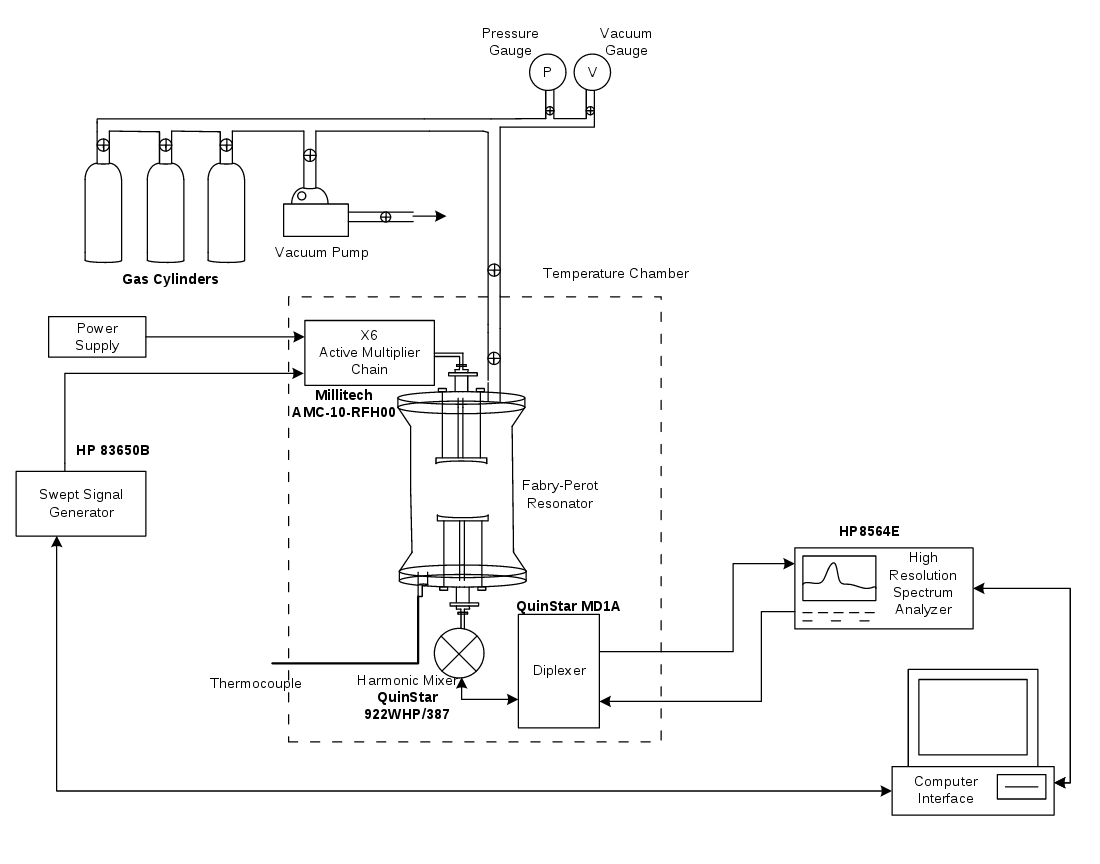
\includegraphics[width=0.7\textwidth]{./images/w-bandsystem.png}
	\caption{Block diagram of the W band measurement system. Solid lines represent the electrical connections and the arrows show the direction of the signal propagation. Valves controlling the flow of gasses are shown by small crossed circles.}
    \label{fig:wbandimage}
\end{figure}


\subsection{F-band Subsystem}
The F-band measurement system is used to measure the 2-3 mm-wavelength properties of sulfur dioxide and is shown in figure \ref{fig:fbandimage}.

The swept signal generator (HP 83650B) is used to generate a signal in the 33-50 GHz range which
is amplified and fed through a frequency tripler. The output of the tripler is fed to the input end of the FPR. The RF signal from the output port of the FPR is fed to a harmonic mixer which can operate with an LO frequency as high as 18 GHz. An external diplexer is used to combine the IF and LO signals. For a particular RF and IF frequency,  the LO frequency can be computed using

\begin{equation} \label{eq:fbandlo}
f_{LO} = \frac{f_{RF} - f_{IF}}{N_H	}
\end{equation}

\noindent where N$_H$ is the lowest integer such that $f_{lo} < 18 GHz$.

\begin{figure}[H]
    \centering
	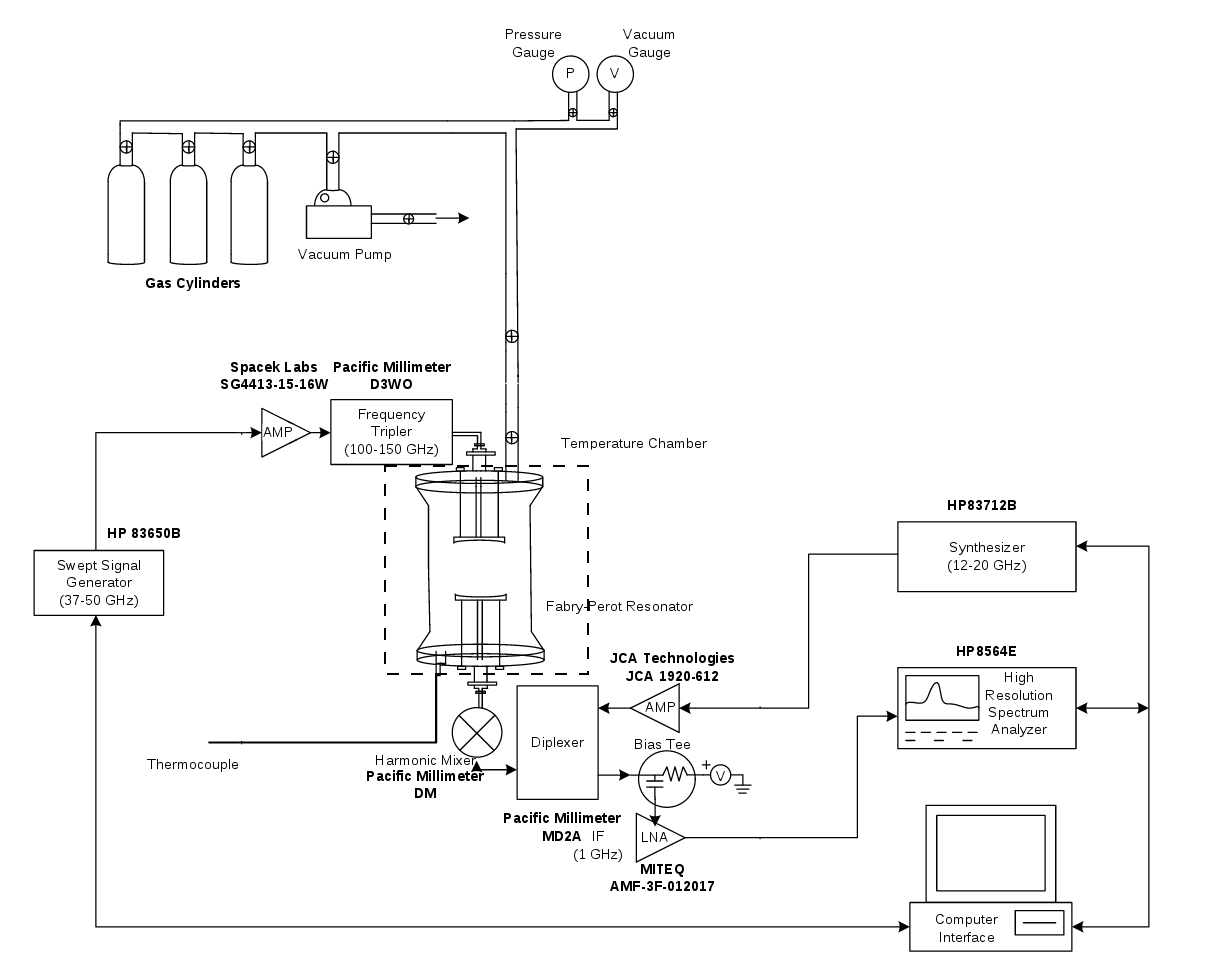
\includegraphics[width=0.7\textwidth]{./images/f-bandsystem.png}
	\caption{Block diagram of the F band measurement system. Solid lines represent the electrical connections and the arrows show the direction of the signal propagation. Valves controlling the flow of gasses are shown by small crossed circles.  }
    \label{fig:fbandimage}
\end{figure}

\section{Data Handling Subsystem}

The data acquisition system consists of a computer connected to the spectrum analyzer (HP 8564E), swept signal generator (HP 83650B), and continuous wave (CW) signal generator (HP 83712B, the local oscillator for the F-Band system) via a general purpose interface bus (GPIB). The instruments are controlled via Matlab script and their appropriate programming language. The software used is similar to Devaraj and Steffes \cite{system-description} \cite{Devaraj-thesis} with modifications for equipment changes.

\section{Measurement Procedure}

The most important prerequisite for performing measurement of gas properties is ensuring a leak-proof system. This is done through two methods, the first is by drawing a vacuum inside the FPR and verifying the integrity of the vacuum over time. The second way is by adding a positive pressure of CO$_2$ to the system and making sure there are no leaks in any of the connectors and valves. Ensuring a leak-proof system allows for not only precise measurements but also ensures no toxic gases are released into the testing environment.

After the system is ensured to be leak-proof and at a stable temperature, a vacuum is drawn and a measurement is taken using the appropriate subsystem (W-band for 3-4 mm-wavelengths, F-band for 2-3 mm-wavelengths). This allows for a base line measurement of the FPR's resonances and the Quality factor. Once this baseline is established the gas under test is added to the system.

Once the gas temperature has stabilized, another set of tests measuring the resonant frequencies along with the quality factors is taken. More gas is added and the procedure is repeated until all suitable pressures are taken. A vacuum is drawn once again but this time it is pumped overnight due to the gas being tested (SO$_2$) and its properties of ``sticking'' (or adsorbing) to metal. Another vacuum measurement is taken to measure any possible system error.

Once the second vacuum measurements are taken CO$_2$ is then added to the chamber until the resonances are matched to the same frequency of our test gas. Again measurements are taken and this is repeated for every pressure of the test gas. Once this is finished a vacuum is again drawn and another test is taken. 

Lastly the system is set up for a transmissivity test where we measure t (equation \ref{eq:t}) for each given resonant frequency. The system is then set back up and is ready for a new test. %Reference table \ref{tab:testmatrix} for the testing matrix being used.

